\documentclass{standalone}
\usepackage{tikz}
\usetikzlibrary{positioning, shapes.misc}

\begin{document}

\begin{tikzpicture}

% Placeholder image
\node[inner sep=0, outer sep=0] (image) at (0,0) {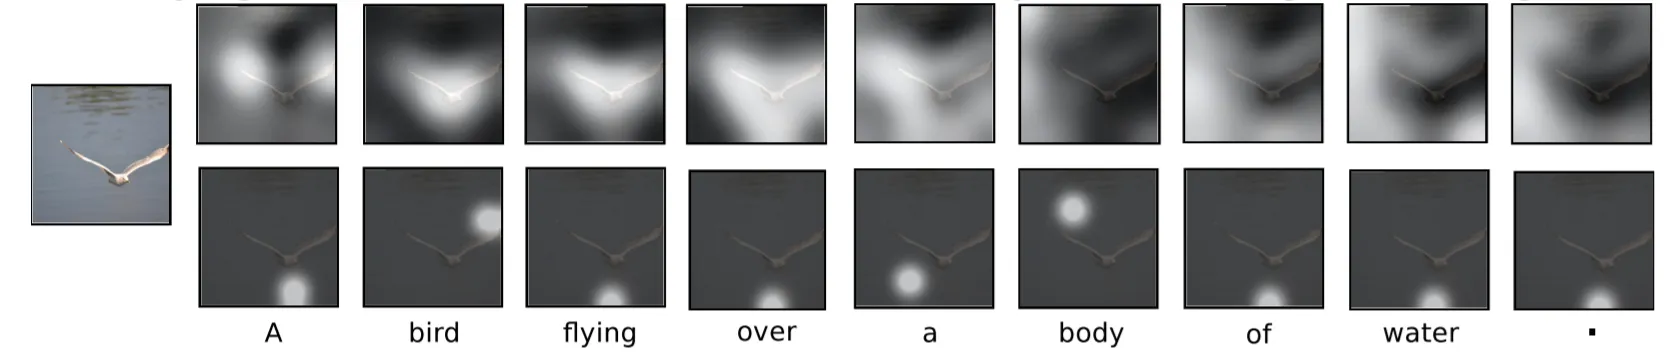
\includegraphics[width=16cm,height=4cm]{tikz/chapter7 - Attention Types.png}};
% \node[fit=(image), draw] {};
\node[fill=white, xshift=-5.35cm, yshift=-1.7cm] (a) {\footnotesize A};
\node[fill=white, xshift=-3.85cm, yshift=-1.7cm] (bird) {\footnotesize bird};
\node[fill=white, xshift=-2.25cm, yshift=-1.715cm] (flying) {\footnotesize flying};
\node[fill=white, xshift=-0.74cm, yshift=-1.715cm] (over) {\footnotesize over};
\node[fill=white, xshift=0.85cm, yshift=-1.715cm] (a2) {\footnotesize a};
\node[fill=white, xshift=2.38cm, yshift=-1.715cm] (body) {\footnotesize body};
\node[fill=white, xshift=3.95cm, yshift=-1.715cm] (of) {\footnotesize of};
\node[fill=white, xshift=5.58cm, yshift=-1.715cm] (water) {\footnotesize water};
\node[fill=white, xshift=7.17cm, yshift=-1.77cm] (tick) {.};

\node[fill=white, xshift=8.45cm, yshift=1.2cm] (soft) {(Soft)};
\node[fill=white, xshift=8.45cm, yshift=-0.7cm] (soft) {(Hard)};

\end{tikzpicture}

\end{document}